\documentclass[10pt]{article}
\usepackage[ruled, linesnumbered]{algorithm2e}
\usepackage{Jan1, epsfig, subfigure, amssymb, multirow, algorithmic,amsmath}
\usepackage{latexsym,amssymb,epsfig,graphicx,subfigure,rotating,multirow,colortbl,xcolor,amsmath,algorithmic,booktabs,url}
\usepackage{accents}
\usepackage{subfig}
\textwidth 160mm
\textheight 215mm
\voffset 1mm
\oddsidemargin 1mm
\evensidemargin 1mm
\newtheorem{definition}{Definition}
\newtheorem{theorem}{Theorem}
\newtheorem{proposition}{Proposition}
\newtheorem{conjecture}{Conjecture}
\newtheorem{corollary}{Corollary}
\newtheorem{lemma}{Lemma}
\newtheorem{example}{Example}


\usepackage[english]{babel}
\usepackage{blindtext}


\title{OpenModelica Solvers}

\author{Anton de Villiers\thanks{HealthQ Technologies, Office 9, First Floor, The Woodmill Lifestyle, Vredenburg Road, Devon Valley,
Stellenbosch, 7600, South Africa}}

\renewcommand{\thefigure}{\arabic{section}.\arabic{figure}}
\renewcommand{\thetable}{\arabic{section}.\arabic{table}}
\begin{document}
\setcounter{page}{1}



\newcommand{\blokkie}{\hspace{.07cm}\Box\hspace{.07cm}}

%%%%% Set up the coloured tables %%%%%
\colorlet{tableheadcolor}{gray!25} % Table header colour = 25% gray
\colorlet{tablerowcolor}{gray!10} % Table row separator colour = 10% gray
\newcommand{\headcol}{\rowcolor{tableheadcolor}}
\newcommand{\rowcol}{\rowcolor{tablerowcolor}}

% The top-most line of a table
\newcommand{\topline}{\arrayrulecolor{black}\specialrule{0.1em}{\abovetopsep}{0pt}%
	\arrayrulecolor{tableheadcolor}\specialrule{\belowrulesep}{0pt}{0pt}%
	\arrayrulecolor{black}}

	% The top-most line of a table
\newcommand{\toplinee}{\arrayrulecolor{black}\specialrule{0.1em}{\abovetopsep}{0pt}%
	\arrayrulecolor{tablerowcolor}\specialrule{\belowrulesep}{0pt}{0pt}%
	\arrayrulecolor{black}}

% The line between the headings and the table body
\newcommand{\midline}{\arrayrulecolor{tableheadcolor}\specialrule{\aboverulesep}{0pt}{0pt}%
	\arrayrulecolor{black}\specialrule{\lightrulewidth}{0pt}{0pt}%
	\arrayrulecolor{white}\specialrule{\belowrulesep}{0pt}{0pt}%
	\arrayrulecolor{black}}

% A line for when the upper row is rowcolor and the next line is white
\newcommand{\midlinecbw}{\arrayrulecolor{tablerowcolor}\specialrule{\aboverulesep}{0pt}{0pt}%
	\arrayrulecolor{black}\specialrule{\lightrulewidth}{0pt}{0pt}%
 	\arrayrulecolor{white}\specialrule{\belowrulesep}{0pt}{0pt}%
	\arrayrulecolor{black}}

% A line with no black, to further separate a rowcolor row and a white row
\newcommand{\midlinecw}{\arrayrulecolor{tablerowcolor}\specialrule{\aboverulesep}{0pt}{0pt}%
	\arrayrulecolor{tablerowcolor}\specialrule{\lightrulewidth}{0pt}{0pt}%
	\arrayrulecolor{white}\specialrule{\belowrulesep}{0pt}{0pt}%
	\arrayrulecolor{black}}

% A line for when the upper row is white and the next line is rowcolor
\newcommand{\midlinewbc}{\arrayrulecolor{white}\specialrule{\aboverulesep}{0pt}{0pt}%
	\arrayrulecolor{black}\specialrule{\lightrulewidth}{0pt}{0pt}%
	\arrayrulecolor{tablerowcolor}\specialrule{\belowrulesep}{0pt}{0pt}%
	\arrayrulecolor{black}}

% sadfsdfsdf sdfsdfsdf
\newcommand{\midlinehr}{\arrayrulecolor{tablerowcolor}\specialrule{\aboverulesep}{0pt}{0pt}%
	\arrayrulecolor{black}\specialrule{\lightrulewidth}{0pt}{0pt}%
	\arrayrulecolor{tableheadcolor}\specialrule{\belowrulesep}{0pt}{0pt}%
	\arrayrulecolor{tablerowcolor}}


% A line for the bottom of the table, when the last row is white
\newcommand{\bottomline}{\arrayrulecolor{white}\specialrule{\aboverulesep}{0pt}{0pt}%
	\arrayrulecolor{black}\specialrule{\heavyrulewidth}{0pt}{\belowbottomsep}}%

% A line for the bottom of the table, when the last row is rowcolor
\newcommand{\bottomlinec}{\arrayrulecolor{tablerowcolor}\specialrule{\aboverulesep}{0pt}{0pt}%
	\arrayrulecolor{black}\specialrule{\heavyrulewidth}{0pt}{\belowbottomsep}}%

\newcommand{\bottomlinect}{\arrayrulecolor{tableheadcolor}\specialrule{\aboverulesep}{0pt}{0pt}%
	\arrayrulecolor{black}\specialrule{\heavyrulewidth}{0pt}{\belowbottomsep}}%
%%%%% Set up the coloured tables %%%%%



\maketitle



\pagestyle{myheadings}


\section{Introduciton}

An ordinary differential equation (ODE) is an equation that involves some ordinary derivatives (as opposed to partial derivatives) of a function. Often, our goal is to solve an ODE, {\em i.e.}\ determine what function or functions satisfy the equation. Implementations of solving ODEs generally involves numerical methods of approximating future state variables, since symbolic approaches may quickly become infeasible.

The quantized state systems (QSS)~\cite{MigoniKofman2009} methods are a family of numerical integration solvers based on the idea of state quantization, dual to the traditional idea of time discretization. Unlike traditional numerical solution methods, which approach the problem by discretizing time and solving for the next (real-valued) state at each successive time step, QSS methods keep time as a continuous entity and instead quantize the system's state, instead solving for the time at which the state deviates from its quantized value by a quantum.

They can also have many advantages compared to classical algorithms. They inherently allow for modeling discontinuities in the system due to their discrete-event nature and asynchronous nature. They also allow for explicit root-finding and detection of zero-crossing using explicit algorithms, avoiding the need for iteration, a fact which is especially important in the case of stiff systems, where traditional time-stepping methods require a heavy computational penalty due to the requirement to implicitly solve for the next system state.

In view of HealthQ's requirements, a Linearly Implicit QSS (LIQSS)~\cite{MigoniKofman2009} numerical solver is to be developed and incorporated within the OpenModelica~\cite{OpenModelica} framework.

\section{Current state of work}

At the moment we have a fully functioning version of a basic LIQSS solver in OpenModelica. The implementation is by no means in a finalized state of operation. There are some known issues that still needs to be addressed and some implementation issues, in OpenModelica, that are being discovered throughout this project.

To incorporate the LIQSS solver, the entire OMCompiler~\cite{OpenModelica} submodule was cloned into a local repository (repo) for development. OMCompiler is coded in {\sf C}, accompanied by some {\sf C++} as well as a scripting language unique to OpenModelica's puposes called {\sf Susan Templating}. The entire repo is necessary as investigation was performed into many different areas of the code within this repo. A new LIQSS solver was added, based on the initial design of the already implemented QSS solver. The solver was tested on a variety of smaller models to ensure that the LIQSS solver would be able to deal with the individual components in isolation. The core test are around the simulation of Valve's (IdealValve's and RegularizedIdealValve's) in the OpenModelica context. Furthermore, the Pulse was also tested. The short-term goal is to successfully simulate the Danielsen Ottesen (Handbook) model. Since the Handbook model contains most of the components that the Virtual Human Model (VHM) contains, the current aim is that the LIQSS solver should work on the VHM if the Handbook model can be simulated successfully.

To compare our numerical results of ODE systems obtained by the LIQSS solver, we compare to our ``gold-standard'' algorithm DASSL~\cite{DASSL}, which is known to deliver expected numerical results. The issues generally arise when solving for certain events as well as very stiff mathematical systems. The problems are often centered around {\sf C} code implementation details or the manner in which events are coded in OpenModelica.




\subsection{Valve}

Table~\ref{tab1} contains the graphical results of the various Valve models under consideration. The DASSL solver can simulate all of these models accurately. The LIQSS solver can solve the model with no valve, as well as the Regularized Valve model given that the step size specified in the solver is small enough. The ideal Valve model cannot be solved by LIQSS in its current form. Instead a different approach is required whereby certain small positive values are tweaked to ensure that the valve closes at the appropriate times. This issue is an implementation consideration that exists with numerical specification in both the LIQSS solver and OpenModelica.

\begin{table}[htbp]
	\centering%\footnotesize
		\begin{tabular}{ccm{6cm}m{6cm}}
    \topline	\headcol
    Valve&& DASSL&LIQSS\\\midline
   1 && 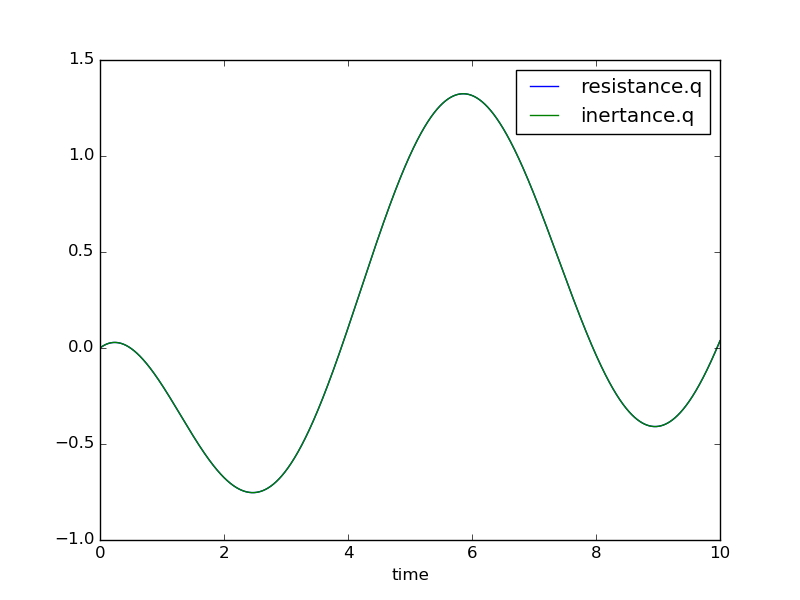
\includegraphics[scale=0.3]{./Figures/DASSL1.png}&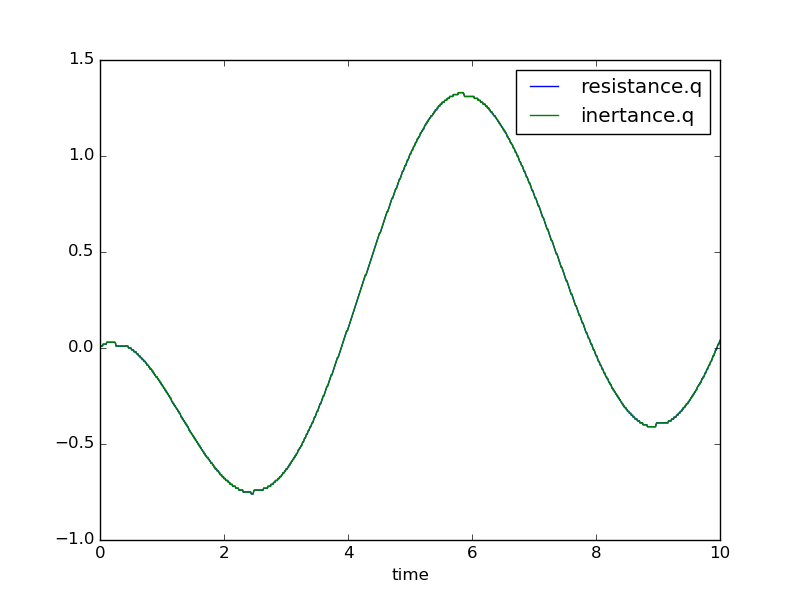
\includegraphics[scale=0.3]{./Figures/LIQSS1.png}\\\rowcol
    2 && 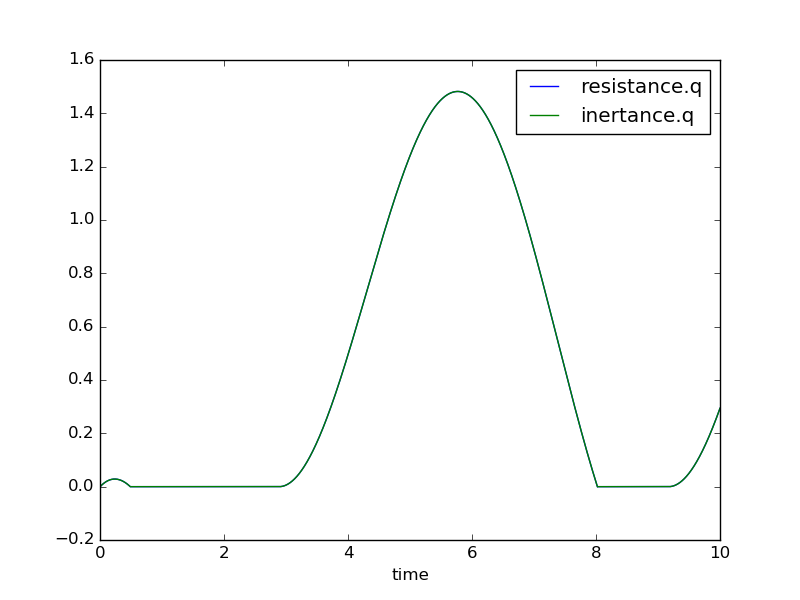
\includegraphics[scale=0.3]{./Figures/DASSL2.png}&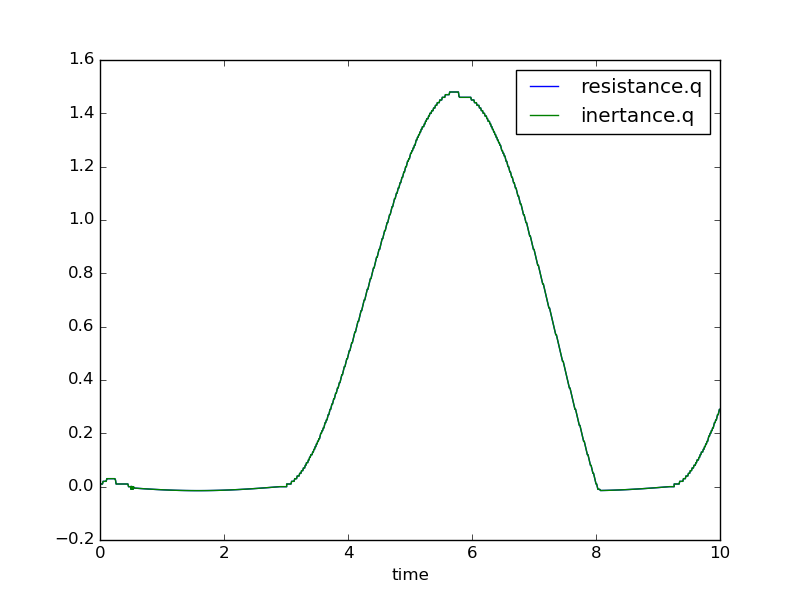
\includegraphics[scale=0.3]{./Figures/LIQSS2.png}\\
    3 && 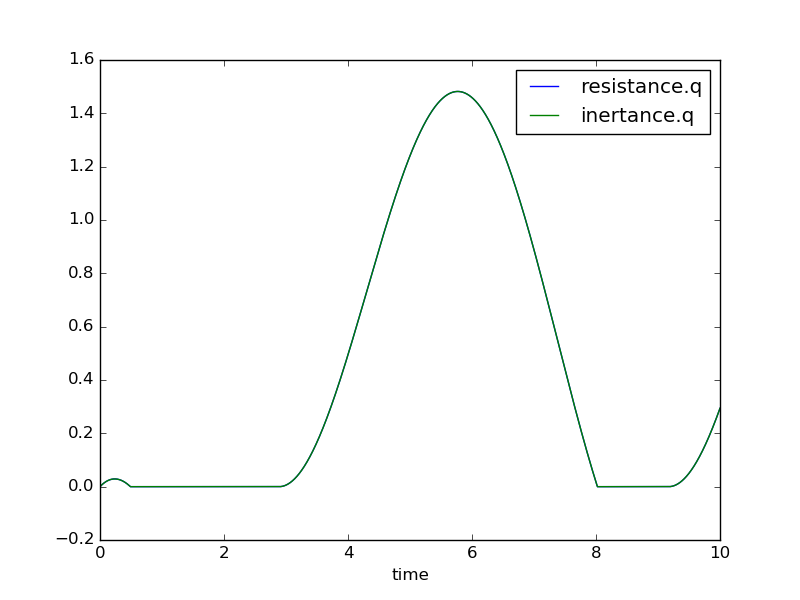
\includegraphics[scale=0.3]{./Figures/DASSL3.png}&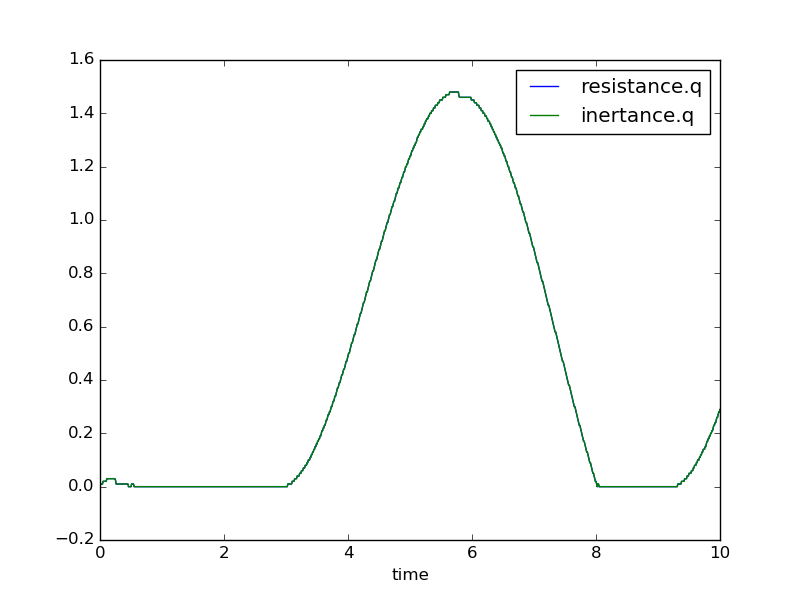
\includegraphics[scale=0.3]{./Figures/LIQSS3.png}\\\bottomlinec
    \end{tabular}


\caption{The graphical results of the Valve simulations. 1) The Base model with no Valve. 2) The Ideal Valve. 3) The Regularized Valve.}
\label{tab1}
    \end{table}


\section{Future implementation tasks}

Current outstanding tasks related to improving the current version of the LIQSS solver is hosted on an Asana account~\cite{asana}. These improvement mainly align with optimizing the code. To summarize some of the most relevant and important outstanding tasks:
\begin{itemize}
 \item To only evaluate the ``affected'' ODEs during each iteration.
 \item Understanding the event handling process in OpenModelica.
 \item Remove unnecessary ODE function calculations.
 \item Incorporating personalized nominal values for all state variables.
 \item Ensuring increases in step sizes are reasonable, not too small and not too large.
 \item Investigate various manners of incorporating nominal values in calculating $\Delta Q_j$ for each state variable $j$.
\end{itemize}

The most recent issues are centered around scripting a manner of flattening the handbook model and adding nominal values.

\section{Impediments}

The main impediment centers around implementations on higher order LIQSS solvers. For an $n$-th order LIQSS solver, we require the symbolic equations of the $n$-th order derivatives of the ODE system. The initial belief was that one could approximate higher order derivatives numerically, but these results may easily become substantially inaccurate as the first order derivatives are based on approximate state variable assignment, which is then in turn used to approximate a higher order derivative value. The effect of the approximation values is thus compounded.

Instead, QSS Solver~\cite{qss} used the {\sf C++} library to symbolically derive functions and thus obtaining higher order ODEs. This library is called {\sf GiNaC}~\cite{ginac}. Although this library has its limitations, it can correctly derive a large subset of function, and by initial guesses it will be able to process the ODE system of the VHM.

The impediment is then to incorporate {\sf GiNaC} into the OpenModelica framework to successfulle derive functions and to the incorporate the derived function in the OpenModelica numerical solvers. This may become a major undertaking as this will essentially entail making notable structural alterations to OpenModelica (and not only the OMCompiler submodule).

\section{The envisioned finished product}

The finished product should be able to simulate the VHM in its entirety. The aim is to have an ODE solver (LIQSS or a higher order version) that can solve the system of ODEs faster than DASSL, while still maintaining accurate numerical results of the ODE system consideration.


{\footnotesize
\begin{thebibliography}{10}

\bibitem{asana}{\sc Asana}, 2016, {\em Asana task management tool}, [Online], Cited 15\textsuperscript{th} March 2016, Available from {\url{https://app.asana.com}}

\bibitem{ginac}{\sc GiNaC}, 2016, {\em GiNaC is not a CAS}, [Online], Cited 15\textsuperscript{th} March 2016, Available from {\url{http://www.ginac.de/}}

\bibitem{OpenModelica} {\sc OpenModelica}, 2016, {\em Open Source Modelica Consortium}, [Online], Cited 15\textsuperscript{th} March 2016, Available from {\url{https://openmodelica.org/}}

\bibitem{OMCompiler} {\sc OMCompiler}, 2016, {\em HealthQ OMCompiler submodule repository}, [Online], Cited 15\textsuperscript{th} March 2016, Available from {\url{https://bitbucket.org/antonpdv/omcompiler}}

\bibitem{MigoniKofman2009} {\sc Migoni G \& Fofman E}, 2009, {\em Linearly implicit discrete event methods for stiff ODE's}, Latin American Applied Research, {\bf{39(3)}}, pp.\, 245--254.

\bibitem{DASSL}{\sc Petzold LR}, 1982, {\em A description of DASSL: A differential/algebraic system solver}, Technical Report, Applied Mathematics Division, Sandia National Laboratories, Livermore (CA).

\bibitem{qss}{\sc QSS Solver}, 2016, {\em Modeling and simulation tool for continuous and hybrid systems}, [Online], Cited 15\textsuperscript{th} March 2016, Available from {\url{https://sourceforge.net/projects/qssengine/}}




\end{thebibliography}}

\end{document}